\newpage 
\ifnum \Version=1
\question[6] Consider the first order system. 
$$\vec x \, ' = A\vec x, \quad A = \begin{pmatrix} 2&1&1\\0&2&0\\1&1&2\end{pmatrix}, \quad \vec x = \vec x(t)  $$
The eigenvalues of $A$ are $\lambda_1 = 1, \lambda_2 = 2$, and $\lambda_3 = 3$. 
\begin{parts}
    \part Determine the eigenvectors of $A$. Please show your work.  \ifnum \Solutions=0 
    \vspace{14cm}
    \fi
    \part Write down the general solution to the system of differential equations using your results from Part (a).
\end{parts}

\ifnum \Solutions=1 {\color{DarkBlue} Solution written below. 
    \begin{figure}[h]
    \centering
    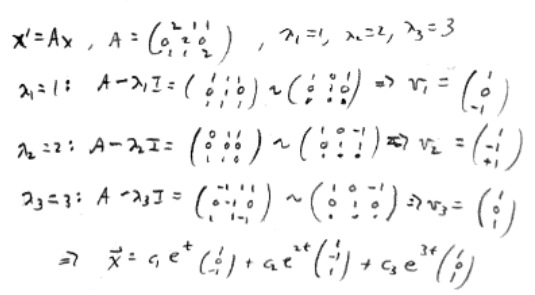
\includegraphics[width=14cm]{Images/ImgTest2System.png}
    \end{figure}  

} 
\else 
\vspace{3cm}
\fi
\fi

\ifnum \Version=2
\question[6] Consider the first order system. 
$$\vec x \, ' = A\vec x, \quad A = \begin{pmatrix} 2&1&1\\1&2&1\\1&1&2\end{pmatrix}, \quad \vec x = \vec x(t)  $$
The eigenvalues of $A$ are $\lambda_1 =\lambda_2 = 1$, and $\lambda_3 = 4$. 
\begin{parts}
    \part Determine the eigenvectors of $A$. Please show your work.  
    \ifnum \Solutions=0 
    \vspace{14cm}
    \fi
    \part Write down the general solution to the system of differential equations using your results from Part (a).
\end{parts}
\ifnum \Solutions=1 {\color{DarkBlue} The eigenvalues for the repeated eigenvalue computed below:
\begin{align}
    \lambda_1 = 1: A - I = \begin{pmatrix} 1&1&1 \\1&1&1\\1&1&1\end{pmatrix}, \quad \Rightarrow \quad v_1 = \begin{pmatrix} 1\\-1\\0\end{pmatrix}, \ v_2 = \begin{pmatrix} 1\\0\\-1\end{pmatrix}
\end{align}
Any two linearly independent vectors in the null space of this matrix is sufficient.  For the remaining matrix we have
\begin{align}
    A - \lambda_3I = \begin{pmatrix} -2&1&1\\1&-2&1\\1&1&-2\end{pmatrix} \sim  \begin{pmatrix} 0&-3&3  \\1&-2&1\\0&-3&3\end{pmatrix}\sim  \begin{pmatrix} 1&-2&1\\0&1&-1\\0&0&0\end{pmatrix}\sim  \begin{pmatrix} 1&0&-1\\0&1&-1\\0&0&0\end{pmatrix} 
\end{align}
Any vector in the null space is sufficient. For example we can choose
\begin{align}
    v_3 = \begin{pmatrix} 1\\1\\1\end{pmatrix}
\end{align}
The general solution is
\begin{align}
    \vec x &= 
    c_1e^{-t}\begin{pmatrix} 1\\-1\\0\end{pmatrix}
    +c_2 e^{-t}\begin{pmatrix} 1\\0\\-1\end{pmatrix}
    +c_3 e^{-4t}\begin{pmatrix} 1\\1\\1\end{pmatrix}
\end{align}
} 
\else 
\vspace{3cm}
\fi
\fi


\ifnum \Version=3
\question[6] Consider the first order system. 
$$\vec x \, ' = A\vec x, \quad A = \begin{pmatrix} 4&1&1\\1&4&1\\1&1&4\end{pmatrix}, \quad \vec x = \vec x(t)  $$
The eigenvalues of $A$ are $\lambda_1 =\lambda_2 = 3$, and $\lambda_3 = 6$. 
\begin{parts}
    \part Determine the eigenvectors of $A$. Please show your work.  
    \ifnum \Solutions=0 
    \vspace{14cm}
    \fi
    \part Write down the general solution to the system of differential equations using your results from Part (a).
\end{parts}
\ifnum \Solutions=1 {\color{DarkBlue} The eigenvalues for the repeated eigenvalue computed below:
\begin{align}
    A - \lambda_1I = \begin{pmatrix} 1&1&1 \\1&1&1\\1&1&1\end{pmatrix}, \quad \Rightarrow \quad v_1 = \begin{pmatrix} 1\\-1\\0\end{pmatrix}, \ v_2 = \begin{pmatrix} 1\\0\\-1\end{pmatrix}
\end{align}
Any two linearly independent vectors in the null space of this matrix is sufficient.  For the remaining matrix we have
\begin{align}
    A - \lambda_3I = \begin{pmatrix} -2&1&1\\1&-2&1\\1&1&-2\end{pmatrix} \sim  \begin{pmatrix} 0&-3&3  \\1&-2&1\\0&-3&3\end{pmatrix}\sim  \begin{pmatrix} 1&-2&1\\0&1&-1\\0&0&0\end{pmatrix}\sim  \begin{pmatrix} 1&0&-1\\0&1&-1\\0&0&0\end{pmatrix} 
\end{align}
Any vector in the null space is sufficient. For example we can choose
\begin{align}
    v_3 = \begin{pmatrix} 1\\1\\1\end{pmatrix}
\end{align}
The general solution is
\begin{align}
    \vec x &= 
    c_1e^{-3t}\begin{pmatrix} 1\\-1\\0\end{pmatrix}
    +c_2 e^{-3t}\begin{pmatrix} 1\\0\\-1\end{pmatrix}
    +c_3 e^{-6t}\begin{pmatrix} 1\\1\\1\end{pmatrix}
\end{align}
} 
\else 
\vspace{3cm}
\fi
\fi





\ifnum \Version=4
\question[6] Consider the first order system. 
$$\vec x \, ' = A\vec x, \quad A = \begin{pmatrix} 2&1&1\\1&2&1\\1&1&2\end{pmatrix}, \quad \vec x = \vec x(t)  $$
The eigenvalues of $A$ are $\lambda_1 =\lambda_2 = 1$, and $\lambda_3 = 4$. 
\begin{parts}
    \part Determine the eigenvectors of $A$. Please show your work.  
    \ifnum \Solutions=0 
    \vspace{14cm}
    \fi
    \part Write down the general solution to the system of differential equations using your results from Part (a).
\end{parts}
\ifnum \Solutions=1 {\color{DarkBlue} The eigenvalues for the repeated eigenvalue computed below:
\begin{align}
    \lambda_1 = 1: A - I = \begin{pmatrix} 1&1&1 \\1&1&1\\1&1&1\end{pmatrix}, \quad \Rightarrow \quad v_1 = \begin{pmatrix} 1\\-1\\0\end{pmatrix}, \ v_2 = \begin{pmatrix} 1\\0\\-1\end{pmatrix}
\end{align}
Any two linearly independent vectors in the null space of this matrix is sufficient.  For the remaining matrix we have
\begin{align}
    A - \lambda_3I = \begin{pmatrix} -2&1&1\\1&-2&1\\1&1&-2\end{pmatrix} \sim  \begin{pmatrix} 0&-3&3  \\1&-2&1\\0&-3&3\end{pmatrix}\sim  \begin{pmatrix} 1&-2&1\\0&1&-1\\0&0&0\end{pmatrix}\sim  \begin{pmatrix} 1&0&-1\\0&1&-1\\0&0&0\end{pmatrix} 
\end{align}
Any vector in the null space is sufficient. For example we can choose
\begin{align}
    v_3 = \begin{pmatrix} 1\\1\\1\end{pmatrix}
\end{align}
The general solution is
\begin{align}
    \vec x &= 
    c_1e^{-t}\begin{pmatrix} 1\\-1\\0\end{pmatrix}
    +c_2 e^{-t}\begin{pmatrix} 1\\0\\-1\end{pmatrix}
    +c_3 e^{-4t}\begin{pmatrix} 1\\1\\1\end{pmatrix}
\end{align}
} 
\else 
\vspace{3cm}
\fi
\fi


\ifnum \Version=5
\question[6] Consider the first order system. 
$$\vec x \, ' = A\vec x, \quad A = \begin{pmatrix} 4&1&1\\1&4&1\\1&1&4\end{pmatrix}, \quad \vec x = \vec x(t)  $$
The eigenvalues of $A$ are $\lambda_1 =\lambda_2 = 3$, and $\lambda_3 = 6$. 
\begin{parts}
    \part Determine the eigenvectors of $A$. Please show your work.  
    \ifnum \Solutions=0 
    \vspace{14cm}
    \fi
    \part Write down the general solution to the system of differential equations using your results from Part (a).
\end{parts}
\ifnum \Solutions=1 {\color{DarkBlue} The eigenvalues for the repeated eigenvalue computed below:
\begin{align}
    \lambda_1 = 1: A - I = \begin{pmatrix} 1&1&1 \\1&1&1\\1&1&1\end{pmatrix}, \quad \Rightarrow \quad v_1 = \begin{pmatrix} 1\\-1\\0\end{pmatrix}, \ v_2 = \begin{pmatrix} 1\\0\\-1\end{pmatrix}
\end{align}
Any two linearly independent vectors in the null space of this matrix is sufficient.  For the remaining matrix we have
\begin{align}
    A - \lambda_3I = \begin{pmatrix} -2&1&1\\1&-2&1\\1&1&-2\end{pmatrix} \sim  \begin{pmatrix} 0&-3&3  \\1&-2&1\\0&-3&3\end{pmatrix}\sim  \begin{pmatrix} 1&-2&1\\0&1&-1\\0&0&0\end{pmatrix}\sim  \begin{pmatrix} 1&0&-1\\0&1&-1\\0&0&0\end{pmatrix} 
\end{align}
Any vector in the null space is sufficient. For example we can choose
\begin{align}
    v_3 = \begin{pmatrix} 1\\1\\1\end{pmatrix}
\end{align}
The general solution is
\begin{align}
    \vec x &= 
    c_1e^{-3t}\begin{pmatrix} 1\\-1\\0\end{pmatrix}
    +c_2 e^{-3t}\begin{pmatrix} 1\\0\\-1\end{pmatrix}
    +c_3 e^{-6t}\begin{pmatrix} 1\\1\\1\end{pmatrix}
\end{align}
} 
\else 
\vspace{3cm}
\fi
\fi



\ifnum \Version=6
\question[4] Consider the first order system. 
$$\vec x \, ' = A\vec x, \quad A = \begin{pmatrix} -3&0&0\\0&-2&-1\\0&1&-2\end{pmatrix}, \quad \vec x = \vec x(t)  $$
The eigenvalues of $A$ are $\lambda_1 = -3$, $\lambda_2 = -2+i$, and $\lambda_3 = -2-i$. 
\begin{parts}
    \part Determine the eigenvectors of $A$. Please show your work.  
    \ifnum \Solutions=0 
    \vspace{14cm}
    \fi
\ifnum \Solutions=1 {\color{DarkBlue} The eigenvalues for the real eigenvalue:
\begin{align}
    \lambda_1 = -3: A + 3I = \begin{pmatrix} 0&0&0\\0&1&-1\\0&1&1\end{pmatrix} \quad \Rightarrow \quad v_1 = \begin{pmatrix} 1\\0\\0\end{pmatrix}
\end{align}
For the complex eigenvalue $\lambda_2$ we have:
\begin{align}
    A - \lambda_2I = 
    \begin{pmatrix} -1-i&0&0\\0&-i&-1\\0&1&-i\end{pmatrix} 
    \sim \begin{pmatrix} 1&0&0\\0&i&1\\0&0&0\end{pmatrix} 
\end{align}
The second row gives us that $ix_2 + x_3 = 0$. Choosing $x_3=i$ we get that $x_2 = -1$. Then an eigenvector is
$$v_2 = \begin{pmatrix} 0\\-1\\i\end{pmatrix} = \begin{pmatrix} 0\\-1\\1\end{pmatrix} + i\begin{pmatrix} 0\\0\\1\end{pmatrix}$$
The eigenvectors are
\begin{align}
    v_1 = \begin{pmatrix} 1\\0\\0\end{pmatrix}, \quad 
    v_2 = \begin{pmatrix} 0\\-1\\i\end{pmatrix} = \begin{pmatrix} 0\\-1\\0\end{pmatrix} + i\begin{pmatrix} 0\\0\\1\end{pmatrix}, \quad 
    v_3 = \begin{pmatrix} 0\\-1\\-i\end{pmatrix} 
\end{align}
Note the following.
\begin{itemize}
    \item Complex eigenvectors come in conjugate pairs, so $v_3 = \bar v_2$. 
    \item Students do not need to write $v_2$ as a combination of two vectors, but it helps when writing the general solution in part b. 
\end{itemize}
} 
\else 
\vspace{3cm}
\fi    
    \part Write down the general solution to the system of differential equations using your results from Part (a).
    
    \ifnum \Solutions=1 {\color{DarkBlue} 
The general solution is
\begin{align}
    \vec x &= 
    c_1 e^{-3t}\begin{pmatrix} 1\\0\\0\end{pmatrix}
    + c_2 e^{-2t} \left( \begin{pmatrix} 0\\-1\\0\end{pmatrix} \cos t - \begin{pmatrix} 0\\0\\1 \end{pmatrix} \sin t \right)
    + c_3 e^{-2t} \left( \begin{pmatrix} 0\\-1\\0\end{pmatrix} \sin t + \begin{pmatrix} 0\\0\\1 \end{pmatrix} \cos t \right)
\end{align}
\newpage
} 
\else 
\vspace{3cm}
\fi
\end{parts}

\fi

\ifnum \Version=7
\question[4] Consider the first order system. 
$$\vec x \, ' = A\vec x, \quad A = \begin{pmatrix} -4&0&0\\0&-3&-1\\0&1&-3\end{pmatrix}, \quad \vec x = \vec x(t)  $$
The eigenvalues of $A$ are $\lambda_1 = -4$, $\lambda_2 = -3+i$, and $\lambda_3 = -3-i$. 
\begin{parts}
    \part Determine the eigenvectors of $A$. Please show your work.  
    \ifnum \Solutions=0 
    \vspace{14cm}
    \fi
\ifnum \Solutions=1 {\color{DarkBlue} The eigenvalues for the real eigenvalue:
\begin{align}
    \lambda_1 = -4: A + 4I = \begin{pmatrix} 0&0&0\\0&1&-1\\0&1&1\end{pmatrix} \quad \Rightarrow \quad v_1 = \begin{pmatrix} 1\\0\\0\end{pmatrix}
\end{align}
For the complex eigenvalue $\lambda_2$ we have:
\begin{align}
    A - \lambda_2I = 
    \begin{pmatrix} -1-i&0&0\\0&-i&-1\\0&1&-i\end{pmatrix} 
    \sim \begin{pmatrix} 1&0&0\\0&i&1\\0&0&0\end{pmatrix} 
\end{align}
The second row gives us that $ix_2 + x_3 = 0$. Choosing $x_3=i$ we get that $x_2 = -1$. Then an eigenvector is
$$v_2 = \begin{pmatrix} 0\\-1\\i\end{pmatrix} = \begin{pmatrix} 0\\-1\\1\end{pmatrix} + i\begin{pmatrix} 0\\0\\1\end{pmatrix}$$
The eigenvectors are
\begin{align}
    v_1 &= \begin{pmatrix} 1\\0\\0\end{pmatrix} \\ 
    v_2 &= \begin{pmatrix} 0\\-1\\i\end{pmatrix} = \begin{pmatrix} 0\\-1\\0\end{pmatrix} + i\begin{pmatrix} 0\\0\\1\end{pmatrix} \\
    v_3 &= \begin{pmatrix} 0\\-1\\-i\end{pmatrix} 
\end{align}
Note the following.
\begin{itemize}
    \item Complex eigenvectors come in conjugate pairs, so $v_3 = \bar v_2$. 
    \item Students do not need to write $v_2$ as a combination of two vectors, but it helps when writing the general solution in part b. 
\end{itemize}
} 
\else 
\vspace{3cm}
\fi    
    \part Write down the general solution to the system of differential equations using your results from Part (a).
    
    \ifnum \Solutions=1 {\color{DarkBlue} 
The general solution is
\begin{align}
    \vec x &= 
    c_1 e^{-4t}\begin{pmatrix} 1\\0\\0\end{pmatrix}
    + c_2 e^{-3t} \left( \begin{pmatrix} 0\\-1\\0\end{pmatrix} \cos t - \begin{pmatrix} 0\\0\\1 \end{pmatrix} \sin t \right)
    + c_3 e^{-3t} \left( \begin{pmatrix} 0\\-1\\0\end{pmatrix} \sin t + \begin{pmatrix} 0\\0\\1 \end{pmatrix} \cos t \right)
\end{align}
} 
\else 
\vspace{3cm}
\fi
\end{parts}

\fi